\chapter{Plotting  \textcolor{red}{(not finished)}}
\vspace*{-1cm}
\begin{flushright}
\texttt{... is worth a thousand words}
\end{flushright}

\lettrine[nindent=0.35em,lhang=0.40,loversize=0.3]{J}{ulia} has a few interesting packages for plotting:

\begin{itemize}
 \item \texttt{PyPlot}\footnote{PyPlot: \url{https://github.com/stevengj/PyPlot.jl}}: provides an interface to Python's MatPlotLib;
 \item \texttt{Gaston}\footnote{Gaston: \url{https://github.com/mbaz/Gaston.jl}}: provides a \texttt{gnuplot} interface to Julia;
 \item \texttt{Gadfly}\footnote{Gadfly: \url{http://dcjones.github.io/Gadfly.jl/}}: ``The Grammar of Graphics'';
 \item \texttt{Winston}\footnote{Winston: \url{https://github.com/nolta/Winston.jl}}: brings the MATLAB syntax to Julia plots.
\end{itemize}

Here we will discuss \texttt{PyPlot} to take advantage of its extensive documentation and large number of users, making it easy to find examples online. 
% Additionally we present \texttt{gnuplot}, which is a traditional and powerful tool for scientific plotting. \texttt{Gnuplot} can be used with Julia via the \texttt{Gaston} package, but we will not cover this package here.

\section{PyPlot}
\label{sec:PyPlot}

\subsection{Installing PyPlot}

To install \texttt{PyPlot}, first you need Python and Matplotlib. If you use Ubuntu Linux, run

\begin{minted}{bash}
 $ sudo apt-get update
 $ sudo apt-get install python python-matplotlib
\end{minted}

Now you can install PyPlot. Start Julia and run: \mintinline[escapeinside=||]{julia}{|\julia| Pkg.add("PyPlot")}.

\subsection{Using PyPlot}

To use \texttt{PyPlot}, first you have to initialize it by calling: \mintinline[escapeinside=||]{julia}{|\julia| using PyPlot}. 

\begin{example}{Using PyPlot}
\begin{minted}{julia}
using PyPlot
x = linspace(-3pi,3pi,200);
plot(x,  sin(x)./x, color="red", linewidth=2.0, linestyle="-");
plot(x, -sin(x)./x, color="blue", linewidth=2.0, linestyle="--");
xlabel("x");
ylabel("f(x)");
\end{minted}
\end{example}

Since the \texttt{PyPlot} package is an interface to Python's Matplotlib, one may use its extensive documentation\footnote{Matplotlib's documentation: \url{http://matplotlib.org/}}.


\subsection{Most useful features and examples}

\subsubsection{Calling non-ported functions from Matplotlib}

PyPlot's documentation says that only the documented Python's \texttt{matplotlib.pyplot} API is exported to Julia. Nonetheless, other functions from Python's \texttt{PyPlot} can be accessed as

\begin{center}
 \texttt{matplotlib.pyplot.foo(...)} $\longrightarrow$ \texttt{plt[:foo](...)},
\end{center} 
where on the left we have Python's notation, and on the right Julia's.

For instance, you can generate an histogram using:

\begin{example}{Using non-ported functions from \texttt{Matplotlib}}
\begin{minted}{julia}
using PyPlot
x = randn(100000);
plt[:hist](x);
xlabel("Random number");
ylabel("Number of occurrences");
\end{minted}
\end{example}

\subsubsection{Latex}

It is very easy to use Latex with Julia's PyPlot package. Implicitly, PyPlot uses the LaTexStrings package\footnote{LaTeXStrings: \url{https://github.com/stevengj/LaTeXStrings.jl}}. Therefore on can use Latex commands on a string simply constructing it prepending with a \texttt{L}. For instance:

\begin{example}{Using Latex}
\begin{minted}[escapeinside=||,breaklines]{julia}
 using PyPlot
 
 x = linspace(0, 2pi, 100);
 f = sin(x);
 
 plot(x, f);
 xlabel(L"$\theta$ [rads]");
 ylabel(L"$\sin\theta$ [a.u.]");
\end{minted}
\end{example}

This Latex notation can be used in all text elements of PyPlot.

\subsubsection{Subplot}

The \texttt{subplot} command allows you to break the plot window into a grid. Say that the desired grid has $N$ lines and $M$ columns, the command \mintinline{julia}{subplot(N, M, j)} specifies that you want to plot the next figure into the $j$-th element of the grid, with the elements sorted in a ``Z'' shape. Try the next example.

\begin{example}{Using subplot}
\begin{minted}[escapeinside=||,breaklines]{julia}
 using PyPlot
 
 x = linspace(-5pi, 5pi, 1000);

 clf();
 
 subplot(2,2,1);
 plot(x, sin(x));
 xlabel(L"$x$");
 ylabel(L"$\sin(x)$");
 
 subplot(2,2,2);
 plot(x, cos(x));
 xlabel(L"$x$");
 ylabel(L"$\cos(x)$");

 subplot(2,2,3);
 plot(x, exp(-x.^2));
 xlabel(L"$x$");
 ylabel(L"Gaussian");
 
 subplot(2,2,4);
 plot(x, sin(x)./x); 
 xlabel(L"$x$");
 ylabel(L"$sinc(x)$");
 
 tight_layout(); # adjust the subplots to better fit the figure

\end{minted}
\end{example}

In the example above we are using Latex notation for the labels. The final command \textbf{tight\_layout(...)} allows you to adjust the subplots spacings to better adjust them within the figure. This avoids overlapping of the labels and plots.

Even more control can be achieved with the command \textbf{subplot2grid(...)}, which we use in Fig.~\ref{fig:FourierSeries}, for instance. Here the shape is passed as a tuple $(N,M)$ to the first parameter, the second parameter takes the location of the desired plot an ordered pair $(i,j)$, where $0 \leq i \leq (N-1)$ and $0 \leq j \leq (M-1)$. The top-left corner grid element is $(i,j) = (0,0)$, and the bottom-right is $(i,j) = (N-1, M-1)$. The \texttt{subplot2grid} becomes more interesting as the next parameters allow you to set a \texttt{rowspan} and a \texttt{colspan} to span over cells. Check again Example \ref{ex:FourierSeries}.


\subsubsection{Labels}

\red{Relevant commands: text}

\subsubsection{Legends}

\red{Relevant commands: legend}

\subsubsection{Other plot elements}

\red{Relevant commands: annotate, arrow, axes, axis, axhline, axvline, contour, }

\subsubsection{Saving into files (PNG, PDF, SVG, EPS, ...)}

Figures are shown by default on screen as PNG. However, you can save it to files with many different formats using the \texttt{savefig(...)} command. Check the example:

\begin{example}{Using subplot}
\begin{minted}[escapeinside=||,breaklines]{julia}
 using PyPlot
 
 x = linspace(-5pi, 5pi, 1000);
 f = sin(x);
 plot(x, f);
 xlabel(L"$\theta$ [rads]");
 ylabel(L"$f(\theta) = \sin\theta$");
 
 savefig("myplot.png");
 savefig("myplot.pdf");
 savefig("myplot.svg");
 savefig("myplot.eps");
\end{minted}
\end{example}

Please check the full documentation of the \texttt{matplotlib} for more details. You can choose the paper size, dpi, etc.

\subsubsection{Animations}

Here's an example of using Julia and \texttt{matplotlib} to create animations\footnote{Adapted from Andee Kaplan's presentation at \url{http://heike.github.io/stat590f/gadfly/andee-graphics/}}. The \texttt{PyCall} package is used to import the \texttt{animation} library from Python, since it is not natively implemented in \texttt{PyPlot}.

\begin{example}{Animated plot}
\begin{minted}[escapeinside=||,breaklines]{julia}
using PyCall # package used to call Python functions
using PyPlot

# import the animation library
@pyimport matplotlib.animation as anim

# this function must plot a frame of the animation
# the parameter t will be iterated by the matplotlib
function animate(t)
  # in this example we willl plot a Gaussian moving around
  c = 3*sin(2pi*t);
  x = linspace(-10, 10, 200);
  y = exp(-(x-c).^2/2);

  # clear the figure before ploting the new frame
  clf(); 
  
  # plot the new frame
  plot(x,y)

  # for this basic usage, the returned value is not important
  return 0
end

# matplotlib's FuncAnimation require an explicit figure object
fig = figure();

tspan = linspace(0, 5, 100); # will be used to iterate the frames

# animation with a interval of 20 miliseconds between frames
video = anim.FuncAnimation(fig, animate, frames=tspan, interval=20)

# save the animation to a MP4 file using ffmpeg and the x264 codec
video[:save]("anim.mp4", extra_args=["-vcodec", "libx264"])
\end{minted}
\end{example}














% \section{Gnuplot \textcolor{red}{(unfinished)}}

\newcounter{gnuplothomework} \newcommand{\gphome}{\begin{large}Homework \arabic{gnuplothomework}\end{large}}
\newcounter{gnuplotexample}  \newcommand{\gpexample}{Example \arabic{gnuplotexample}}

% \vspace*{-1cm}
% \begin{flushright}
% \texttt{set term classnotes}
% \end{flushright}

Gnuplot is a tradicional, very useful and powerful tool for scientific plot. It can be used either for quick plots to visualize data, or to obtain fine figures for reports and publications. Gnuplot's current version at the time I'm writing these notes is \texttt{5.0}, and it can be found on the webpage \url{www.gnuplot.info}. There one also finds an extensive User Manual. In this chapter we elaborate on the main aspects of \texttt{gnuplot} to introduce the language and capabilities of this fantastic tool for the students.

\subsection{Installing gnuplot}

\subsection*{Debian/Ubuntu Linux}

Most Linux distributions have \texttt{gnuplot} in their repositories. If you use Ubuntu, you can install from the terminal with the commands:

\begin{example}{Installing gnuplot in Ubuntu Linux}
\begin{minted}[]{bash}
 sudo apt-get update
 sudo apt-get install gnuplot # this installs gnuplot version 4.6.6
 # or...
 sudo apt-get install gnuplot5 # this installs gnuplot version 5.0
 sudo apt-get install gnuplot-mode # To install gnuplot emacs mode
\end{minted}
\end{example}

If you use the \texttt{Emacs} text editor, the \texttt{gnuplot-mode} package above provides a full IDE for \texttt{gnuplot} within \texttt{Emacs}.

\subsection*{MS Windows and Apple OS X}

I highly recommend you to use \texttt{Linux}. However, if you are stubborn enough I allow you to waste time with another OS. If you have an Apple computer (at least that's UNIX-based) you can install \texttt{gnuplot} via \texttt{homebrew}\footnote{Homebrew: \url{brew.sh}.} or \texttt{MacPorts}\footnote{MacPorts: \url{www.macports.org}.}. If you use Windows (really?)... good luck!


\subsection{The command line interface}

\texttt{Gnuplot} runs on the command line, there's no GUI. If you really like graphical interfaces, please check \texttt{QtiPlot}\footnote{QtiPlot: \url{www.qtiplot.com}.}. To start \texttt{gnuplot} (in \texttt{Linux}) open the terminal, type \texttt{gnuplot} and press Enter... you will see this interface:

\begin{example}{Gnuplot's initial screen}
\begin{minted}{bash}
        G N U P L O T                                                                                                             
        Version 5.0 patchlevel 1    last modified 2015-06-07                                                                      
                                                                                                                                  
        Copyright (C) 1986-1993, 1998, 2004, 2007-2015                                                                                
        Thomas Williams, Colin Kelley and many others

        gnuplot home:     http://www.gnuplot.info
        faq, bugs, etc:   type "help FAQ"
        immediate help:   type "help"  (plot window: hit 'h')

Terminal type set to 'qt'
gnuplot> 
\end{minted}
\end{example}

From the start it tells you that if you need help, just type \texttt{help}. In \texttt{gnuplot} this is extremely useful, as it comes with an extensive and well written documentation. Therefore, let's start with the most important command: \mintinline[escapeinside=||]{gnuplot}{|gnuplot>| help plot}. Read it! Check and test the examples by yourself.

In the examples you will see that you can call sine and cosine functions natively. Actually, \texttt{gnuplot} supports all functions from the Unix math library. When in doubt try common names for the functions. For instance, let's try to plot a Gaussian:

\begin{example}{Plotting Gaussians with gnuplot}
\begin{minted}[escapeinside=||]{gnuplot}
 |gnuplot>| w = 2.0; # set variable w to store the Gaussian width
 |gnuplot>| set xrange [-10:10]; # set the range of horizontal axes
 |gnuplot>| f(x)=exp(-0.5*(x/w)**2); # define a Gaussian function
 |gnuplot>| plot f(x); # plot f(x)
 |gnuplot>| plot f(x), f(x-1); # plot two functions
\end{minted}
\end{example}

Try to run this example line-by-line in \texttt{gnuplot}. If all goes well you should get Fig.~\ref{fig:gnuplotgaussian}. Excellent! Now you understand how the \texttt{gnuplot} interface works and you made your first plot. Play around and try to plot other functions, change the axes range and read again the plot help to see what you can do. By default you are probably using the `qt' terminal, which allows you to save, copy and print your figure from the plot window.

\begin{figure}[ht!]
 \centering
 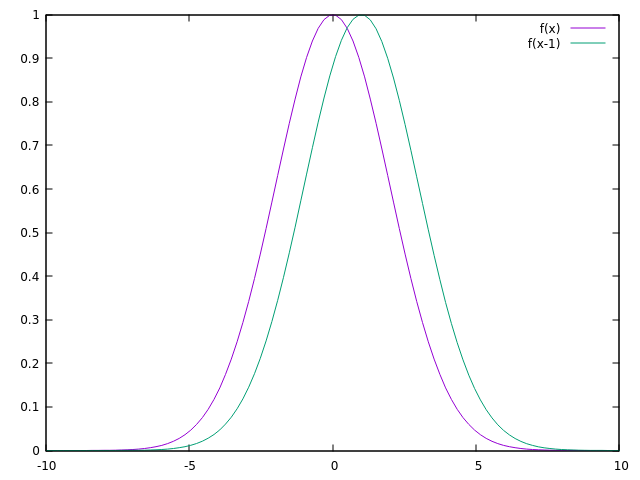
\includegraphics[width=0.5\textwidth]{gnuplot-gaussian.png}
 \caption{Plot of Gaussian functions in \texttt{gnuplot}.}
 \label{fig:gnuplotgaussian}
\end{figure}

\subsection{Using a script file}

While the command line interface is very useful for quick plots, for final figures you will probably need to customize colors, styles, sizes, labels... this can be easily accomplished using a script file, which is simply a text file containing all the commands you want to run. Using your favorite text editor create a file \texttt{gaussian.gp} with the content:

\begin{example}{gnuplot script file `gaussian.gp'}
\begin{minted}[]{gnuplot}
  reset; # cleans the variables and functions
  w = 2.0; # set variable w to store the Gaussian width
  f(x)=exp(-0.5*(x/w)**2); # define a Gaussian function
  set xrange [-10:10]; # set the range of horizontal axes
  set yrange [-0.1:1.1]; # set the range of vertical axes
  set title 'Gaussians'
  set xlabel 'here goes x'
  set ylabel 'here goes f(x)'
  plot f(x) lw 4, f(x-1) lw 2; # plot two functions
\end{minted}
\end{example}

From the \texttt{gnuplot} interface call: \mintinline[escapeinside=||]{gnuplot}{|gnuplot>| load 'gaussian.gp'}. It will open a plot window similar to the previous one, check the differences to understand the new commands on the example.

\subsection{The terminals}

\subsubsection{Example script: epslatex}

\subsection{Using gnuplot with Julia}

\subsection{Most useful commands and examples}

% \section{Another choice: Asymptote}


